\section{Fresnel zones}\label{sec:fresnel}
Taking into account that the application at hand involves radio communication, it is important to mention Fresnel zones. The Fresnel zone is the area around the visual line-of-sight where radio waves spread out into ellipse shaped areas when they leave the antenna. Thus, in figure \ref{fig:3fresnel_zones} three Fresnel zones are stretched between two antennas. 

\begin{figure}[H]
	\centering
	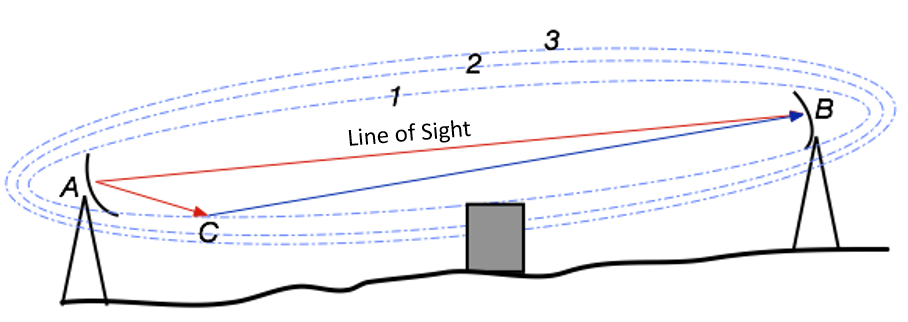
\includegraphics[scale=0.65]{figures/fresnel_zones.png}
	\caption{Fresnel zones between transmitter and receiver}
	\label{fig:3fresnel_zones}
\end{figure}

The figure above shows three examples of Fresnel zones, but there is an infinite number of them. The first zone is the one that has most effect on the performance of the Wireless Network. If there are any obstructions, such as buildings, trees or hills, in the first Fresnel zone, the signal will be affected by them and, consequently, would be weaker at the receiver.

Therefore, it is essential to keep the first Fresnel zone clear of obstruction when planning wireless links. However, it is impractical to avoid 100$\%$ of the obstructions in the real-life. Thus, based on (\hl{refhereimportant})27.maj 09:36, at least 60 $\%$ of the signal should be clear of obstructions. However, to get optimum performance it is recommended to keep the signal 20$\%$ or less blocked.

\subsection{Fresnel zone calculations}
The figure \ref{fig:fresnel_zones} represents the first Fresnel zone between the antennas on the buildings A and B. The radius \textit{r} corresponds to the radius of the Fresnel zone at the point P. 

\begin{figure}[H]
	\centering
	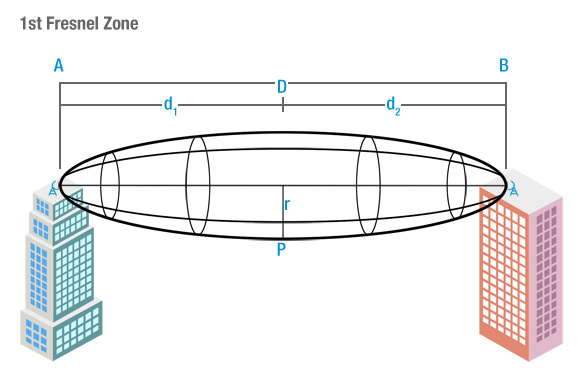
\includegraphics[scale=0.70]{figures/fresnel_zone.jpg}
	\caption{Fresnel zones}
	\label{fig:fresnel_zones}
\end{figure} 

Using the equation \ref{fresnel_zone_cal}, it is possible to calculate the radius, $r_n$, of the nth Fresnel zone at any point P, depending on the wavelength of the transmitted signal, $\lambda$. Thus, $d_1$ and $d_2$ represent the distances between the point P and the antennas A and B, respectively, in figure \ref{fig:fresnel_zones}.

\begin{align}
r_n = \sqrt{\frac{n \lambda d_1 d_2}{d_1+d_2}} \label{fresnel_zone_cal}
\end{align}

On the other hand, it is often useful to know the maximum radius of the zone. The radius of the Fresnel zone achieves its maximum when both distances $d_1$ and $d_2$ have the same size ($d_1=d_2$, which means that $d_1+d_2=D$). Based on the relation between the wavelength and the frequency, $\lambda = \frac{c}{f}$, and on the equation \ref{fresnel_zone_cal}, the radius of the first Fresnel zone can be calculated using the equation \ref{eq:fresnel_radius3}. In this equation, the frequency, $f$, is in gigahertz, and the total distance, $D$, is in kilometres in order to calculate the radius, $r$, in metres.

\begin{align}
r_1 = \sqrt{\frac{c}{f}\frac{d_1 d_2}{d_1+d_2}} = \sqrt{\frac{c}{f}\frac{d^2}{2d}}, d_1=d_2=d \label{eq:fresnel_radius1}
\end{align}

\begin{align}
r_1 = \sqrt{\frac{c}{2}}\sqrt{\frac{d}{f}} = \sqrt{\frac{c}{4}}\sqrt{\frac{D}{f}}, d=\frac{D}{2} \label{eq:fresnel_radius2}
\end{align}

\begin{align}
r_1 = 8.657 \sqrt{\frac{D}{f}} \label{eq:fresnel_radius3}
\end{align}

\subsection{Fresnel Zones examples without curvature of the earth}
In equation \ref{eq:fresnel_radius3}, by changing the distance between the antennas, $D$, it is clear that the radius, $r$, of the Fresnel zone will also change. In this subsection, there are three examples and some parameters are changed in order to analyse the behaviour of the radius' size. In the following examples, a frequency of 2.4 Ghz is used but the curvature of the earth is not considered. 

The first example shows an antenna and a UA at a height of 20 and 100 meters, respectively, and the distance between them is 10km.

\begin{figure}[H]
	\centering
	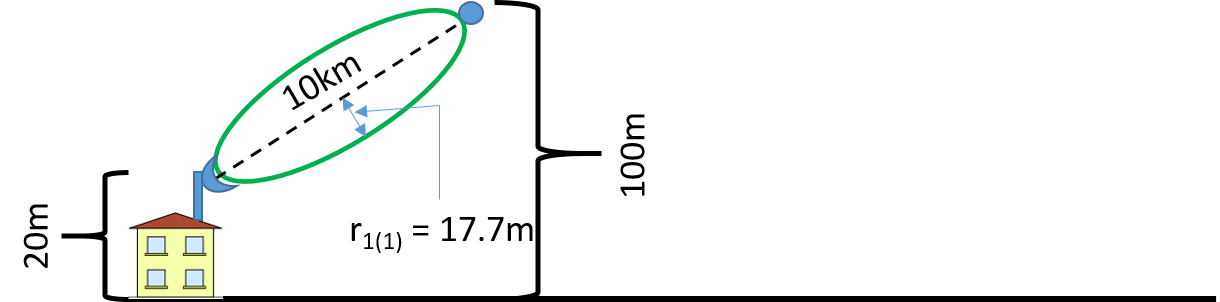
\includegraphics[scale=0.50]{figures/fresnel_10km.png}
	\caption{Fresnel zone when the distance between the transmitter and the receiver is 10km}
	\label{fig:fresnel_zones_10km}
\end{figure}  

In this first example, the radius is:
\begin{align*}
r_1 = 8.657 \sqrt{\frac{10}{2.4}} = 17.7m
\end{align*}

In the second example, the antenna and the UA keep at the same height as before but the distance between them is 20km.

\begin{figure}[H]
	\centering
	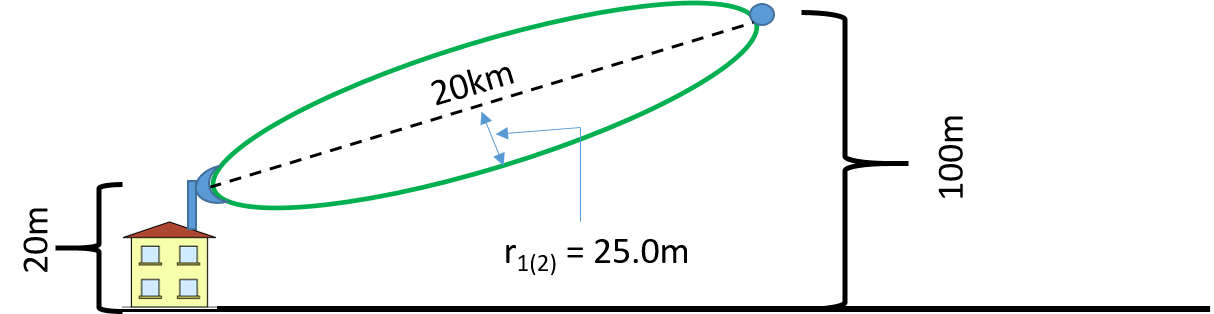
\includegraphics[scale=0.50]{figures/fresnel_20km.png}
	\caption{Fresnel zone when the distance between the transmitter and the receiver is 20km}
	\label{fig:fresnel_zones_20km}
\end{figure}  

The calculated radius is:
\begin{align*}
r_1 = 8.657 \sqrt{\frac{20}{2.4}} = 25.0m
\end{align*}

In the last example of this subsection, the antenna and the UA keep at the same height as in the previous examples but the distance between them is 50km.

\begin{figure}[H]
	\centering
	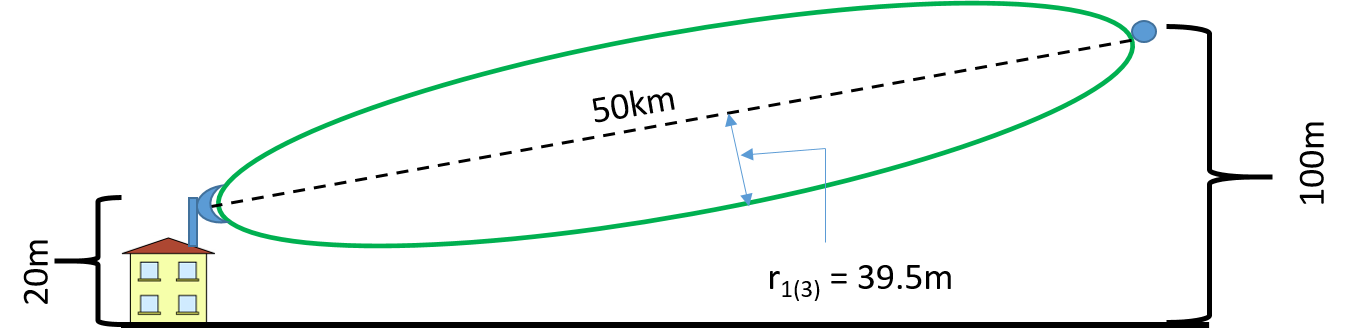
\includegraphics[scale=0.50]{figures/fresnel_50km.png}
	\caption{Fresnel zone when the distance between the transmitter and the receiver is 50km}
	\label{fig:fresnel_zones_50km}
\end{figure}  

In the last case, the calculated radius is:
\begin{align*}
r_1 = 8.657\sqrt{\frac{50}{2.4}} = 39.5m
\end{align*}

In these examples it is demonstrated that the radius of the Fresnel zone increases when the distance between the antennas increases.

\subsection{60$\%$ Clearance Zone of the first Fresnel zone}
As was described in the beginning of this section, it is difficult to have a first Fresnel zone without any obstructions. However, a percentage of obstruction equal or smaller than 40$\%$ makes the connection possible between the transmitter and the receiver.

In this subsection, some examples will demonstrate how tall a structure can be at the center of the first Fresnel zone, taking into account the 60$\%$ clearance. In order to be able to do the calculations the equation \ref{eq:60_percent_radius} was used.

\begin{align}
r_1 = 8.657\sqrt{\frac{0.6D}{f}}\label{eq:60_percent_radius}
\end{align}

For an ideal case, assuming that both antennas are at a height of 20 meters (operating at 2.6GHz) and the distance between them is 10km, the radius is given by the equation \ref{eq:100_distance10}.

\begin{align}
r_1 = 8.657\sqrt{\frac{10}{2.4}} = 17.7m\label{eq:100_distance10}
\end{align}

In this case, the first Fresnel zone would pass just 2.3 meters above the ground level in the middle of the link. 

\begin{figure}[H]
	\centering
	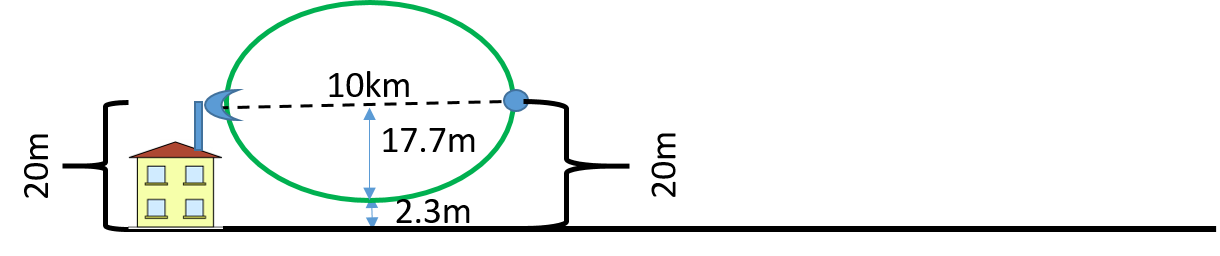
\includegraphics[scale=0.50]{figures/fresnel_10km_height.png}
	\caption{Fresnel zone when the antennas have the same height (20 meters) and when the distance between them is 10km.}
	\label{fig:fresnel_zones_10km_height}
\end{figure}  

In order to calculate how tall a structure should be, it is necessary to calculate the radius of the Fresnel zone when the signal is 60$\%$ cleared (equation \ref{eq:60_distance10}).

\begin{align}
r_{1(60\%)} = 8.657\sqrt{0.6 \frac{10}{2.4}} = 13.7m\label{eq:60_distance10}
\end{align}
  
Therefore, knowing that the height of the longitudinal axis of the ellipsoid is the same as the one of both antennas, it is possible to calculate the maximum altitude of the obstruction. This altitude can be obtained by subtracting the antenna height with the radius calculated in equation \ref{eq:60_distance10}.

\begin{align}
\text{Maximum Obstruction Height} = 20 - 13.7 = 6.3m\label{eq:height_obstruction}
\end{align}

Hence, for this specific example, the maximum tolerated height of any obstruction located in the middle point between both antennas is 6.3m. An illustration of this situation is shown in figure \ref{fig:fresnel_zones_10km_60procent}.

\begin{figure}[H]
	\centering
	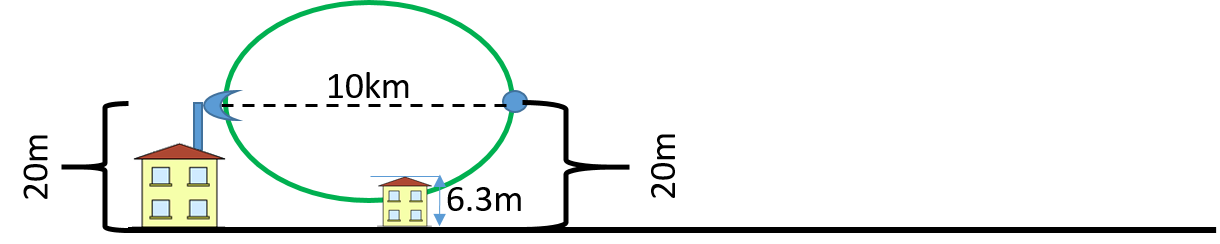
\includegraphics[scale=0.50]{figures/fresnel_10km_60procent.png}
	\caption{Fresnel zone with a 40$\%$ of the signal is blocked.}
	\label{fig:fresnel_zones_10km_60procent}
\end{figure}  

An obstruction higher than 6.3m will give less than 60$\%$ clearance of the Fresnel zone. To prevent this problem, the antenna need to be positioned higher up, the frequency could be changed or the direction of the link should be changed to avoid obstacles.

\subsection{Fresnel zones examples with curvature of the earth}
For longer distance links the curvature of the earth comes into play and may become an obstruction into the Fresnel zone, causing signal losses. Moreover, the longer the distance between the antennas, the greater the radius of the Fresnel zones. Equation \ref{eartheffect} allows to calculate the height difference of Earth's Curvature, $H$, at the mid-point between the two antennas. In order to do the previous calculation, it is necessary to include one parameter related to the total distance between both antennas, $D$ (km), and one related to the effective radius of Earth, $E_r = 8 504 km$.

Furthermore, figure \ref{fig:fresnel_50km_curvature} is an illustration where the curvature of the earth is taking into account. On this figure the antennas on the building and the UA are at 77m height and the distance between them is 50km. 

\begin{align}
H = \frac{1000\cdot D^2}{8\cdot E_r}\label{eartheffect}
\end{align}

\begin{figure}[H]
	\centering
	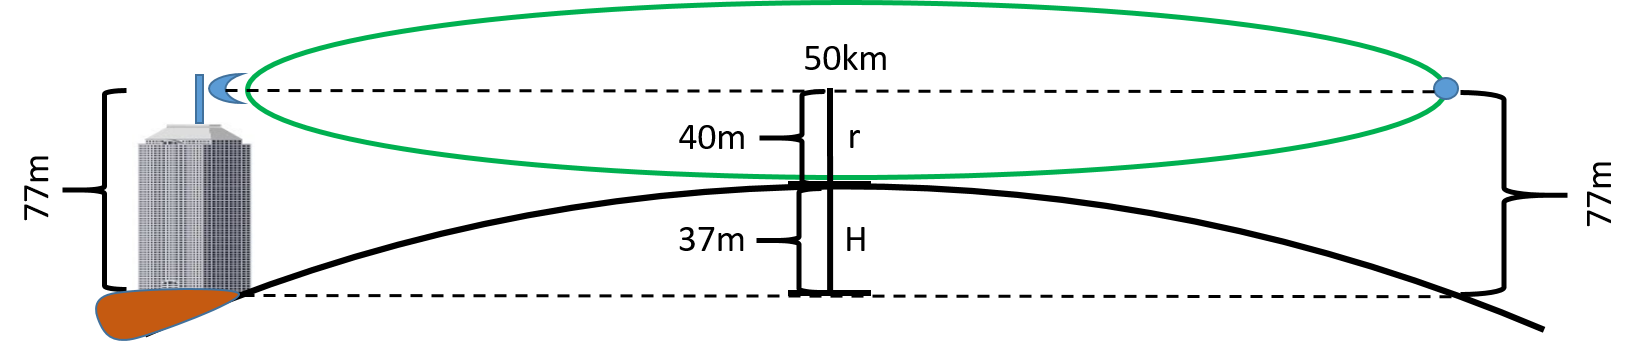
\includegraphics[scale=0.50]{figures/fresnel_50km_curvature.png}
	\caption{Fresnel zone in 50km distance with curvature of the earth taken into account.}
	\label{fig:fresnel_50km_curvature}
\end{figure}

Based on equation \ref{eartheffect}, the height difference of the earth's curvature at the mid-point between the UA and the building:
\begin{align}
\text{H} = \frac{1000 D^2}{8 \cdot E_r} = \frac{1000 \cdot 50^2}{8\cdot 8504} = 36.7m \approx 37m 
\end{align}

Furthermore, the radius of the first Fresnel zone:
\begin{align*}
\text{r} = 8.657\cdot \frac{0.6\cdot D}{f} = 8.657\cdot \frac{50}{2.4} = 39.5m \approx 40m 
\end{align*}

On the other hand, the maximum height of the obstruction between the two devices within the 60$\%$ clearance zone can be calculated with the equations \ref{radius_60}, \ref{Obs_max_height} and \ref{height_max_with_curv}. These calculations are illustrated on figure \ref{fig:fresnel_50km_curvature_obstacle}.

\begin{align}
r_{1(60\%)} &= 8.657\cdot \frac{0.6\cdot D}{f} = 8.657\cdot \frac{0.6\cdot 50}{2.4} = 30.6m \approx 31m \label{radius_60}
\end{align}

The maximum height of the obstruction with the curvature of the earth included:
\begin{align}
\text{Obs}_{\text{max height}} &= 77m - r_{1(60\%)} = 77m - 31m = 46m \label{Obs_max_height}
\end{align}

The actual maximum height of the obstruction:
\begin{align}
\text{height}_{\text{max with curv}} &= \text{Obs}_{\text{max height}} - H = 46m - 37m = 9m\label{height_max_with_curv}
\end{align}

\begin{figure}[H]
	\centering
	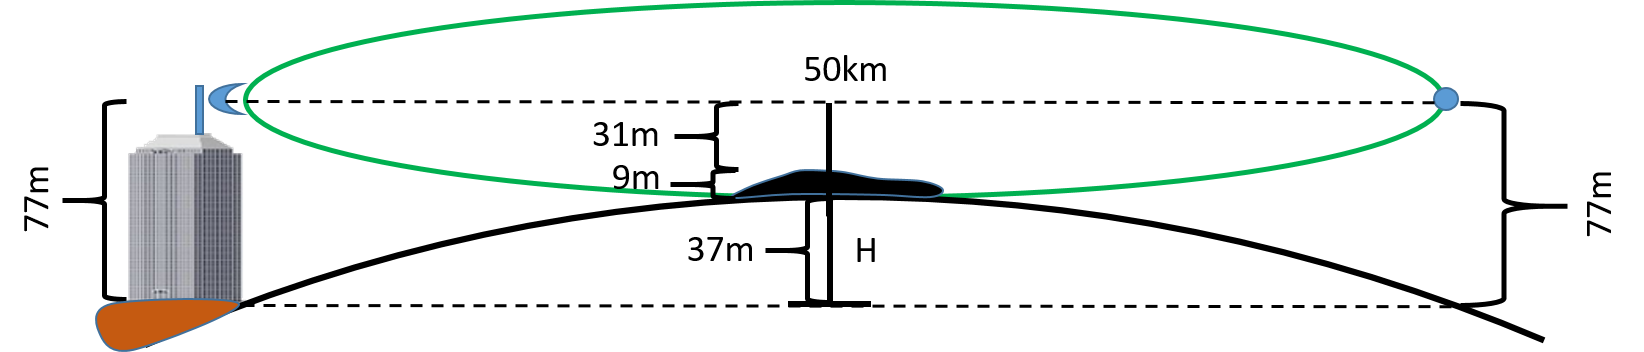
\includegraphics[scale=0.50]{figures/fresnel_50km_curvature_obstacle.png}
	\caption{Fresnel zone taking into account the curvature of the earth and the 60$\%$ clearance.}
	\label{fig:fresnel_50km_curvature_obstacle}
\end{figure}  

Figure \ref{fig:fresnel_50km_curvature_obstacle} shows that it's important to consider the curvature of the earth. Here the obstruction can only be at the height of 9m, since the curvature is an obstruction itself and takes 37m. However, it is important to note that this example only implies when the longitudinal axis of the ellipsoid is the same as the one of both antennas. But nonetheless it gives a good understanding that the Fresnel zones are important factors when building a wireless link network.
